\documentclass[twocolumn, 10pt]{article}

\usepackage{geometry}
\geometry{
	a4paper,
	total={6.85in, 9.92in},
	left=0.71in,
	top=0.63in,
}
\usepackage{caption}
\usepackage{enumitem}
\usepackage[utf8]{inputenc}
\usepackage{hyperref}
\usepackage{graphicx}
\usepackage{listings}
\usepackage{lipsum} % XXX: Remove that
\usepackage{titlesec}
\usepackage{url}
\usepackage{xcolor} % XXX: Remove that
% \usepackage{newunicodechar}

% unicodes styling
% \DeclareUnicodeCharacter{2014}{\dash}
% unicodes - end
\pagenumbering{gobble}

% listing styling
\definecolor{commentsColor}{rgb}{0.497495, 0.497587, 0.497464}
\definecolor{identifierColor}{rgb}{0.9, 0.01, 0.9}
\definecolor{keywordsColor}{rgb}{0.000000, 0.000000, 0.635294}
\definecolor{stringColor}{rgb}{0.558215, 0.000000, 0.135316}

\lstset{
    abovecaptionskip=\vspace{-4pt},
    belowcaptionskip=\vspace{0pt},
    backgroundcolor=\color{yellow!10},
    basicstyle=\ttfamily\tiny,
    breakatwhitespace=true,
    breaklines=true,
    postbreak=\mbox{\textcolor{red}{$\hookrightarrow$}\space},
    commentstyle=\color{commentsColor}\textit,
    caption={},
    escapeinside={\%*}{*)},
    extendedchars=false,
    frame=single,
    frameround=tftf,
    framerule=0pt,
    framexbottommargin=0pt,
    framextopmargin=0pt,
    framexleftmargin=0pt,
    ndkeywordstyle=\color{identifierColor}\bfseries,
    inputencoding=utf8,
    keywordstyle=\color{keywordsColor}\bfseries,
    language=bash,
    % numbers=right,
    % numberstyle=\footnotesize,
    % numberstyle=\tiny\color{commentsColor}, 
    rulecolor=\color{black!30},
    stringstyle=\color{stringColor}\bfseries,
    showspaces=false,
    tabsize=2,
    title=\lstname,
  breaklines=true,
  postbreak=\mbox{\textcolor{red}{$\hookrightarrow$}\space},
}

\lstdefinestyle{c}{language=c,
    morekeywords={uint32_t, int32_t, uint8_t, printf, size_t},
        backgroundcolor=\color{clr-background},
        basicstyle=\color{clr-text}, % any text
        stringstyle=\color{clr-string},
        identifierstyle=\color{clr-variable}, % about not directive, comment, string or known type
        commentstyle=\color{clr-comment},
        directivestyle=\color{clr-preprocessor}, % preprocessor commands
        % listings doesn't differentiate between types and keywords (e.g. int vs return)
        % use the user types color
        keywordstyle=\color{clr-type},
        keywordstyle={[2]\color{clr-constant}}, % you'll need to define these or use a custom language
        tabsize=2
}
\lstdefinestyle{sh}{
  language=sh
}

\lstdefinestyle{json}{language=json,
  morekeywords={uint32_t, int32_t, uint8_t, printf, size_t},
      backgroundcolor=\color{clr-background},
      basicstyle=\color{clr-text}, % any text
      stringstyle=\color{clr-string},
      identifierstyle=\color{clr-variable}, % about not directive, comment, string or known type
      commentstyle=\color{clr-comment},
      directivestyle=\color{clr-preprocessor}, % preprocessor commands
      % listings doesn't differentiate between types and keywords (e.g. int vs return)
      % use the user types color
      keywordstyle=\color{clr-type},
      keywordstyle={[2]\color{clr-constant}}, % you'll need to define these or use a custom language
      tabsize=2
}
\DeclareCaptionFormat{listing}{\rule{]\dimexpr\textwidth+17pt\relax}{0.4pt}\vskip1pt#1#2#3}
% listing - end
\usepackage{etoolbox}
\patchcmd{\thebibliography}{\subsection*{\refname}}{}{}{}

\titlespacing{\section}{0pt}{\parskip}{-\parskip}
\titlespacing{\subsection}{0pt}{\parskip}{-\parskip}

\vspace{-\baselineskip}
\setlength{\parindent}{0pt}
\DeclareCaptionLabelFormat{filelabel}{File~#2}
\captionsetup[lstlisting]{labelformat=filelabel}

\title{RPI4 remote debug recipe!}
\author{Kajetan Brzuszczak}

\makeatletter
\newcommand{\fsize}{\f@size pt }
\newcommand{\textFontName}{\f@family}
\renewcommand{\maketitle}{
\begin{flushleft}
{\noindent\Huge\bf\@title}\break
\end{flushleft}
}
\makeatother

\begin{document}
\maketitle

Tools: \textit{RPI4, C++, VSCode, CMake, Linux}

\subsection*{Minimal project structure}
Replace the following paths with your own favorite paths:
\small
\begin{enumerate}
  \item \textit{/mnt/d/programming/remote\_debug\_rpi/} - workspace
  \item \textit{/mnt/d/programming/x-compile-os/} - image directory
\end{enumerate}

\small

Verify whether your file structure follows the following graph:
\begin{lstlisting}[language=txt,backgroundcolor=\color{gray!10},caption={}]
.
-> .vscode
   -> launch.json
   -> settings.json
-> src
    -> main.cc
-> CMakeLists.txt
-> rpi4.toolchain.cmake
-> build_rpi.sh
\end{lstlisting}

Once you got it, fill up each file with a proper content

% \textit{}
\tiny{}File: launch.json\small{}
\begin{lstlisting}[language=sh,caption={},breaklines=true,literate={,}{,\allowbreak}1]
{"version":"0.2.0", "configurations":[{"name":"RPI 4 - attach", "type":"gdb", "target":"192.168.0.21:9999", "request":"attach", "remote":true,"cwd":"${workspaceRoot}", "gdbpath":"gdb-multiarch", "executable":"out_rpi/debug_rpi", "debugger_args":["--nh", "-iex", "set solib-search-path /mnt/d/programming/remote_debug_rpi/out_rpi", "-iex", "set architecture aarch64", "-iex", "set sysroot /mnt/d/programming/x-compile-os/rpi4"]}]}
\end{lstlisting}

\tiny{}File: settings.json\small{}
\begin{lstlisting}[language=json,breaklines=true,caption={}]
{"clangd.arguments": ["--compile-commands-dir=out_rpi"]}
\end{lstlisting}

\tiny{}File: main.cc\small{}
\begin{lstlisting}[language=c,caption={}]
#include <iostream>
int main(int argc, char* argv[]) {
  auto msg{argc == 2 ? argv[1] : ""};
  std::cout << "msg: " << msg << "\n";
}
\end{lstlisting}

\tiny{}File: CMakeLists.txt\small{}
\begin{lstlisting}[language=sh,breaklines=true,caption={}]
cmake_minimum_required(VERSION 3.26)
project(debug_rpi)
add_executable(debug_rpi src/main.cc)
set_target_properties(debug_rpi PROPERTIES CXX_STANDARD 20 CXX_STANDARD_REQUIRED True)
\end{lstlisting}
  
\tiny{}File: rpi4.toolchain.cmake\small{}
\begin{lstlisting}[language=sh,breaklines=true,caption={}]
set(CMAKE_SYSTEM_NAME Linux)
set(CMAKE_SYSTEM_PROCESSOR arm)
set(CMAKE_SYSROOT /mnt/d/programming/x-compile-os/rpi4)
set(CMAKE_C_COMPILER /usr/bin/aarch64-linux-gnu-gcc-10)
set(CMAKE_CXX_COMPILER /usr/bin/aarch64-linux-gnu-g++-10)
set(CMAKE_FIND_ROOT_PATH_MODE_PROGRAM NEVER)
set(CMAKE_FIND_ROOT_PATH_MODE_LIBRARY ONLY)
set(CMAKE_FIND_ROOT_PATH_MODE_INCLUDE ONLY)
set(CMAKE_FIND_ROOT_PATH_MODE_PACKAGE ONLY)
\end{lstlisting}
% backgroundcolor=\color{yellow!10}
  
\tiny{}File: build\_rpi.sh\small{}
\begin{lstlisting}[language=sh,breaklines=true,caption={}]
cmake -S . -B out_rpi -DCMAKE_EXPORT_COMPILE_COMMANDS=True -DCMAKE_BUILD_TYPE=Debug --toolchain rpi4.toolchain.cmake
cmake --build out_rpi -j7
\end{lstlisting}

\begin{figure}
  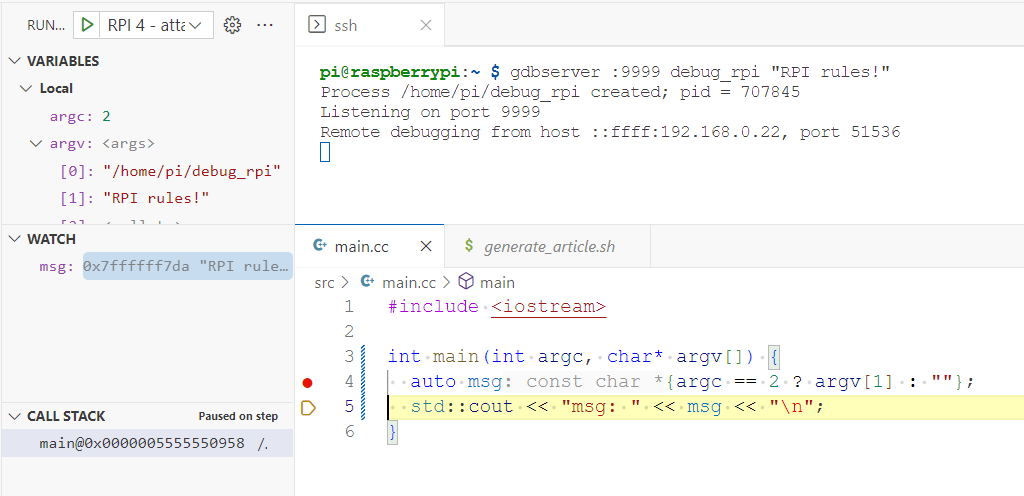
\includegraphics[width=\linewidth]{res/remote_debug_rpi_light.png}
  \caption*{VSCode attached to a remote app}
  \label{fig:debug}
\end{figure}

\subsection*{Environment}
Installing x-compile and indexing tools 
\begin{lstlisting}[backgroundcolor=\color{gray!10},caption={}]
sudo apt install -y gcc-10-aarch64-linux-gnu g++-10-aarch64-linux-gnu gdb-multiarch clangd
\end{lstlisting}

Dump your RPI SD card or download a proper flash image\cite{bib:rpi_images}.
Then we are ready to configure your system and install plugin for debugging

\begin{lstlisting}[language=sh,backgroundcolor=\color{gray!10},breaklines=true,escapechar=|,caption={}]]
wget https://downloads.raspberrypi.org/raspios_lite_arm64/ images/raspios_lite_arm64-2023-05-03/ 2023-05-03-raspios-bullseye-arm64-lite.img.xz
unxz --keep 2023-05-03-raspios-bullseye-arm64-lite.img.xz
mkdir -p /mnt/d/programming/x-compile-os/rpi4
sudo mount -v -o  offset=272629760  2023-05-03-raspios-bullseye-arm64-lite.img /mnt/d/programming/x-compile-os/rpi4

code --install-extension webfreak.debug 
code --install-extension llvm-vs-code-extensions.vscode-clangd
\end{lstlisting}


\subsection*{Playground}
It is time to compile the project and put the binary on the raspberry.
\begin{lstlisting}[language=sh,breaklines=true,caption={},,escapechar=|,backgroundcolor=\color{gray!10}]
./build_rpi.sh
scp out_rpi/debug_rpi rpi:|$\sim$|/ 
\end{lstlisting}

The final step is to run the binary using \textit{gdbserver}, and after that, run a debug session by attaching it in your VSCode (or bye pressing the "\textbf{F5}" key).
\begin{lstlisting}[language=sh,breaklines=true,caption={},escapechar=|,backgroundcolor=\color{gray!10}]
# FROM RPI 
gdbserver :9999 |$\sim$|/debug_rpi
\end{lstlisting}
Voilà! You are now a driver.

\subsection*{Further steps}
Being in sync with the image and the RPI is highly recommended.
  If any library is installed directly on the RPI, the image
  should be updated with the same copy.
\\
With the current setup, you also get automatically generated \textit
  {compile\_commands.json} file utilized by \textit{clangd}
  \cite{bib:clangd} which provides code navigation and code completion, The same approach is appliccable even for quite large repositories,
  such as Chromium.
\\
Last but not least, a major gain of remote debugging is reducing
  the required disk usage by using \textit{stripped} binaries on the RPI while keeping a debuggable version on your PC.
\\
Until platform-spefic header are used f.e. \textit{linux/spi.h} 
  \textit{linux/gpio.h}, you can compile the code locally without additional changes.

\subsection*{Misses}
\begin{enumerate}
  \item rpi ip - hardcoded, seems the plugin does not support aliases
  \item port 9999 - I like this one, but your firewall can have different feelings
  \item mounting offset - check it\cite{bib:mounting-approach} out
\end{enumerate}

\subsection*{Caveats}
Things are gettting much more complicated when project grows larger,
  libraries are distributed more widely, and it is compiled on a remote
  station using a virtual machine (e.g. \textit{qemu}). Eventually, your simple configuration may stop working.
  GDB provides commands that can help point to the correct libraries, 
  such as \textit{set solib-search-path path} or
  \textit{set substitute-path from to} etc.


\subsection*{References}
\begin{enumerate}[label={[\arabic*]}]
  \tiny
  \bibitem{bib:example} Example \url{https://github.com/HalfInner/remote_debug_rpi}
  \bibitem{bib:c++-rpi} \url{https://tttapa.github.io/Pages/Raspberry-Pi/C++-Development-RPiOS/index.html}
  \bibitem{bib:rpi-images} \url{https://www.raspberrypi.com/software/operating-systems/}
  \bibitem{bib:clangd} \url{https://clangd.llvm.org/}
  \bibitem{bib:mounting-approach} \url{https://raspberrypi.stackexchange.com/a/13138}
  \bibitem{bib:gdb-remote-debug} \url{https://developers.redhat.com/blog/2015/04/28/remote-debugging-with-gdb}
\end{enumerate}


\end{document}
